\section{Dijeljeni kod i ulazni podaci}

Kod u nastavku je zajednički za oba algoritma tj. nema veze s samim algoritmom već služi za dohvat podataka i spremanje rezultata algoritma. Sastoji se od metoda za čitanje datoteka s informacijama o oblacima točaka i metoda za spremanje transformacijskih matrica u datoteke. 

\begin{listing}[h!]
  \begin{minted}[frame=lines, linenos]{text}
typedef PointXYZ PT;
typedef PointCloud<PT> PointCloudType;
typedef IterativeClosestPoint<PT, PT, double> ICP;

PointCloudType::Ptr cloud_ref(new PointCloudType());
PointCloudType::Ptr cloud_target(new PointCloudType());
PointCloudType::Ptr cloud_reg(new PointCloudType());

PointCloudType::Ptr cloud_ref_f(new PointCloudType());
PointCloudType::Ptr cloud_target_f(new PointCloudType());

string root_point_clouds = "\\point_clouds\\";
string root_results = "\\icp_results\\";
  \end{minted}
  \caption{Generalizirani ICP - konstante}
  \label{coderef:gen_icp_const}
\end{listing}

U primjeru izvornoga koda \ref{coderef:gen_icp_const} su definirane konstante poput putanje za spremanje rezultata i putanje s ulaznim datotekama. Također su definirani tipovi točaka \mintinline{text}{PT} kao \mintinline{text}{PointXYZ} koje će algoritam koristit te sadrže samo x, y i z koordinate. Mogu se koristiti i drugi oblici točaka. Oblak točaka \mintinline{text}{PointCloudType} je definiran kao kolekcija prethodno definiranih točaka. Naposljetku se definira tip \mintinline{text}{ICP} algoritma tj. s kojim tipovima podataka radi. Definiran je pomoću uređene trojke \mintinline{text}{<PT, PT, double>} što znači da uspoređuje točke tipa \mintinline{text}{PT}, a rezultate u transformacijsku matricu zapisuje kao \mintinline{text}{double} vrijednosti tj. kao brojeve s pomičnim zarezom dvostruke preciznosti.

Definirane su i varijable \mintinline{text}{cloud_ref} koja pokazuje na referentni skup točaka, \mintinline{text}{cloud_target} koja pokazuje na ciljni skup točaka i \mintinline{text}{cloud_reg} koja pokazuje na aproksimiran skup točaka nakon poravnanja. Za algoritme koji koriste filrirane oblake točaka koriste se varijable \mintinline{text}{cloud_ref_f} i \mintinline{text}{cloud_target_f}. One su tipa \mintinline{text}{boost::shared_ptr} te se kao takve predaju metodama kao pokazivači.

\begin{listing}[h!]
  \begin{minted}[frame=lines, linenos]{text}
ICP setupICP() {
 ICP icp;
 icp.setMaxCorrespondenceDistance(0.05);
 icp.setMaximumIterations(500);
 icp.setTransformationEpsilon(1e-8);
 icp.setEuclideanFitnessEpsilon(1);
 return icp;
}
  \end{minted}
  \caption{Instance ICP algoritma}
  \label{coderef:gen_icp_def}
\end{listing}
\pagebreak
U primjeru \ref{coderef:gen_icp_def} se definira ICP algoritam tako da mu se predaju uvjeti zaustavljanja te ostali parametri. Trenutno su zadana tri uvjeta zaustavljanja, a oni su:

\begin{enumerate}
  \item \mintinline{text}{setMaxCorrespondenceDistance} - uzima u obzir samo točke unutar zadanoga promjera u metrima
  \item \mintinline{text}{setMaximumIterations} - maksimalan broj iteracija prilikom estimacije tarnsformacije za neku točku
  \item \mintinline{text}{setTransformationEpsilon} - maksimalna dozvoljena pogreška
\end{enumerate}

\begin{listing}[h!]
  \begin{minted}[frame=lines, linenos]{text}
vector<path> get_files() {
 vector<path> paths;
 path p(root_point_clouds);
 directory_iterator end_itr;
 for (directory_iterator itr(p); itr != end_itr; ++itr) {
  if (is_regular_file(itr->path())) {
   paths.push_back(itr->path());
  }
 }
 return paths;
}
  \end{minted}
  \caption{Skupljanje ulaznih datoteka}
  \label{coderef:gen_icp_collect_files}
\end{listing}
\pagebreak
Kod u primjeru \ref{coderef:gen_icp_collect_files} koristi metode biblioteke Boost\cite{boost} za iteriranje datoteka sa skupovima točaka te vrača vektora s njihovim putanjama. Kod za stvaranje grafova je jednak bez obzira na korišteni algoritam. Grafovi su stvoreni pomoću jezika Kotlin i biblioteke XCharts. Podaci koji vizualiziraju su usporedbe stvarnih podataka tj. referentnih i podataka dobivenih pomoću algoritama. S obzirom da nam algoritmi kao izlaz daju samo transformacijske matrice, potrebno je nekako te matrice prikazati kao koordinate lokacija i kuteve rotacija.

\begin{listing}[h!]
  \begin{minted}[frame=lines, linenos]{text}
fun calculatePointsExperimental(
 icp: List<TransformMatrix>,
 first: Transform
): List<Array<DoubleArray>> {
   val transformations = mutableListOf(pointToMat(first))
   val last = transformations.last()
   icp.forEach { transform ->
    val result = mult(last, transform.matrix)
    transformations.add(result)
   }
  return transformations
}
  \end{minted}
  \caption{Generiranje estimiranih transformacijskih matrica}
  \label{kotlin:gen_est_loc}
\end{listing}

\begin{listing}[h!]
  \begin{minted}[frame=lines, linenos, escapeinside=!!]{text}
fun pointToMat(first:  Transform): Array<DoubleArray> {
 val rot = first.rotation
 val loc = first.location
 val rx = rot.toRx()
 val ry = rot.toRy()
 val rz = rot.toRz()
 val res = multi(rz, multi(ry, rx)) !\label{lineref:multiply_matrices_xyz}!
 return arrayOf(
  arrayOf(res[0][0], res[0][1], res[0][2], loc.x),
  arrayOf(res[1][0], res[1][1], res[1][2], loc.y),
  arrayOf(res[2][0], res[2][1], res[2][2], loc.z),
  arrayOf(0.0, 0.0, 0.0, 1.0)
 )
}
  \end{minted}
  \caption{Generiranje estimiranih lokacija}
  \label{kotlin:init_mat_method}
\end{listing}

Kod u primjeru \ref{kotlin:gen_est_loc} se vidi metoda za generiranje estimiranih točaka iz prve referentne točke i transformacijskih matrica. Kao argumente metoda prima listu transformacijskih matrica \mintinline{text}{icp} te transformaciju prve referentne točke. Algoritam radi tako da prvo izračuna transforamcijsku matricu iz prve referentne točke pomoću metode \ref{kotlin:init_mat_method}. Zapravo se rotacija iz Eulerovog oblika pretvara u zasebne rotacijske matrice te njih pomnoži redosljedom XYZ zbog redosljeda rotacija prilikom ICP estimacije transformacije oblaka točaka. Izgledi pojedinih matrica su prikazani u poglavlju Referentni podaci. Tada se vraća matricu veličine 4x4 koja se sastoji od rotacijske matrice i lokacija. Algoritam koristi prethodno estimiranu transformacijsku matricu te trenutnu estimiranu transformacijsku matricu tako da iz pomnoži pravilima množenja matrica. Tada se dobije nova matrica koja zapravo predstavlja nove koordinate i nove rotacije naspram prethodne. Na liniji \ref{lineref:multiply_matrices_xyz} primjera \ref{kotlin:gen_est_loc} se vidi kako se zapravo primjenjuje formula $R = R_{z}(\gamma)R_{y}(\beta)R_{x}(\alpha)$. Taj redosljed množenja matrica rotacija je vrlo bitan.

Vizualizacije referentnih podataka za oba primjera kretanja vozila možemo vidjeti na sljedećim grafovima. Na njima svaka točka predstavlja jedno očitanje. Slika \ref{fig:gt1_lokacija} prikazuje graf lokacija vozila. Slika \ref{fig:gt1_lokacija_koord} pokazuje koordinate vozila u vremenu. Možemo vidjeti da se mijenjaju samo x i y koordinate zato što vozilo može samo skretati. Slika \ref{fig:gt1_rot_vr} prikazuje valjanje, poniranje i skretanje oko statičnih osi vozila u vremenu. Također se može uoćiti da se samo skretanje mijenja zato što se vozilo ne može valjati niti ponirati. Slika \ref{fig:gt1_rot_kv} također pokazuje rotaciju vozila u vremenu ali predstavljenu u obliku kvaterniona.
\pagebreak
\subsubsection{Primjer referentnih podataka A}
Prvi skup podataka se sastoji od 300 očitanja tj. postoji 300 datoteka sa skupovima točaka. Duljina trajanja te simulacije je 200 sekundi. Parametri koji su korišteni u python skripti za postavljanje lidar senzora su sljedeći:
\begin{enumerate}
  \item Maksimalna udaljenost laserske zrake je postavljena na 1500 cm tj. 15 metara
  \item Maksimalan skup točaka u jednome očitanju je postavljen na 600 000.
\end{enumerate}
\begin{figure}[H]
  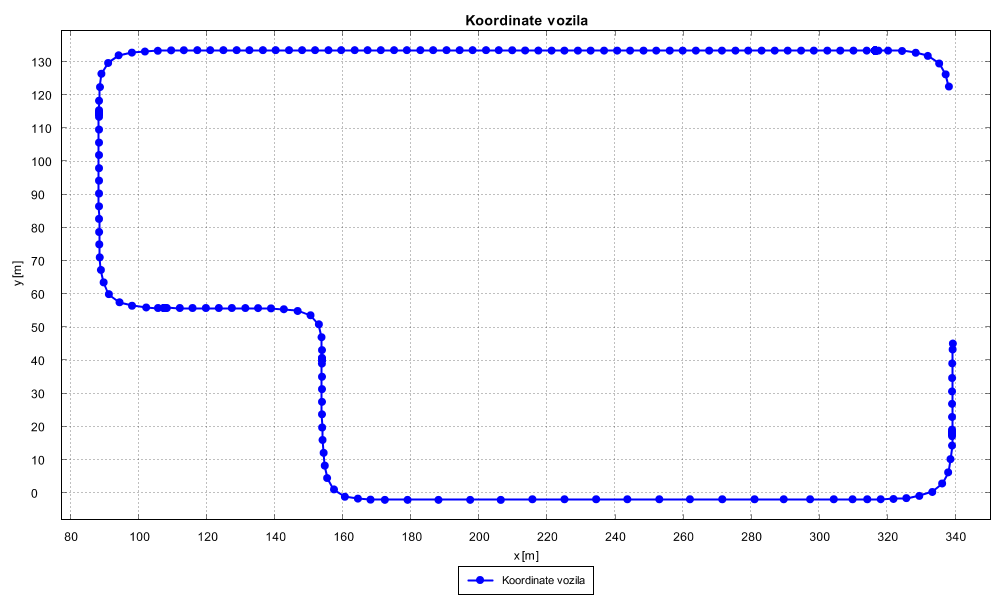
\includegraphics[scale=0.4]{images/koordinate1.png}
  \caption{Graf lokacije vozila}
  \label{fig:gt1_lokacija}
\end{figure}
\begin{figure}[H]
  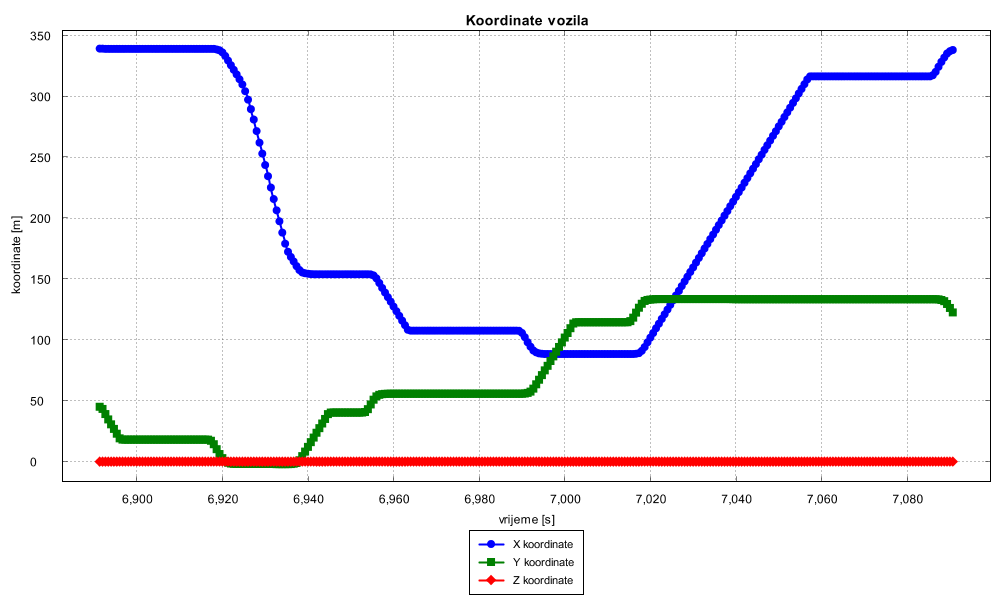
\includegraphics[scale=0.4]{images/koordinate_vrijeme1.png}
  \caption{Graf x, y i z koordinata vozila u vremenu}
  \label{fig:gt1_lokacija_koord}
\end{figure}
\begin{figure}[H]
  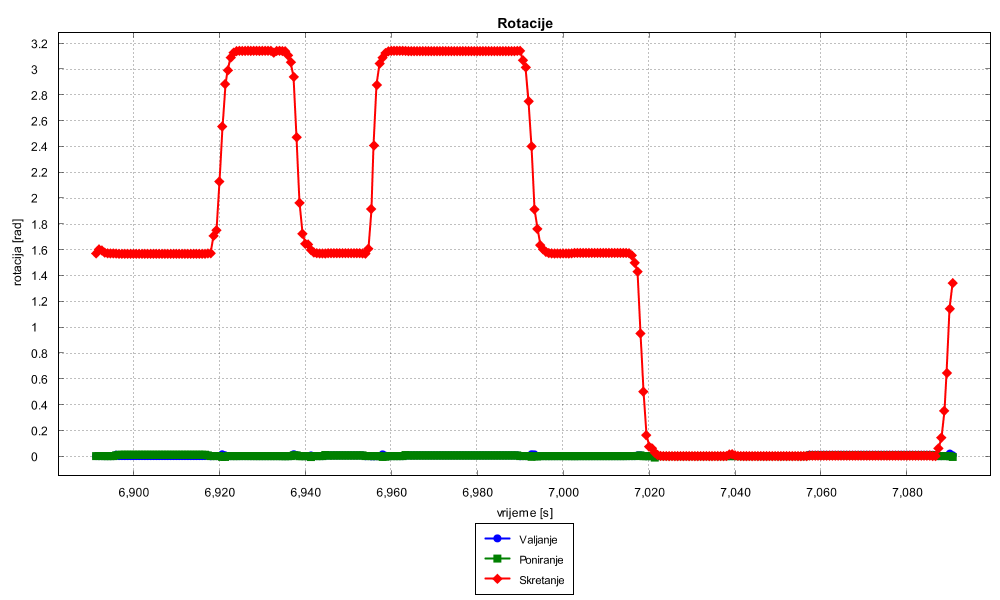
\includegraphics[scale=0.4]{images/rotacija_vrijeme1.png}
  \caption{Valjanje, skretanje i poniranje vozila u vremenu}
  \label{fig:gt1_rot_vr}
\end{figure}
\begin{figure}[H]
  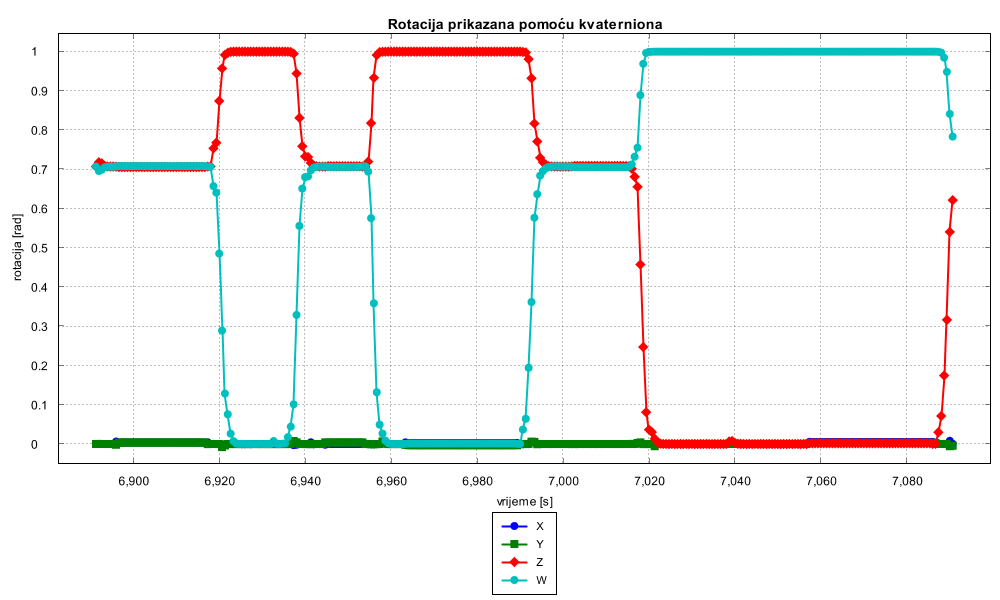
\includegraphics[scale=0.4]{images/rotacija_kvaterni1.png}
  \caption{Rotacija vozila u obliku kvaterniona}
  \label{fig:gt1_rot_kv}
\end{figure}

\newpage
\subsubsection{Primjer referentnih podataka B}
Drugi skup podataka se sastoji od 600 očitanja tj. postoji 600 datoteka sa skupovima točaka. Duljina trajanja te simulacije je 80 sekundi. Parametri koji su korišteni u python skripti za postavljanje lidar senzora su sljedeći:
\begin{enumerate}
  \item Maksimalna udaljenost laserske zrake je postavljena na 2000 cm tj. 20 metara
  \item Maksimalan skup točaka u jednome očitanju je postavljen na 1 000 000.
\end{enumerate}
\begin{figure}[H]
  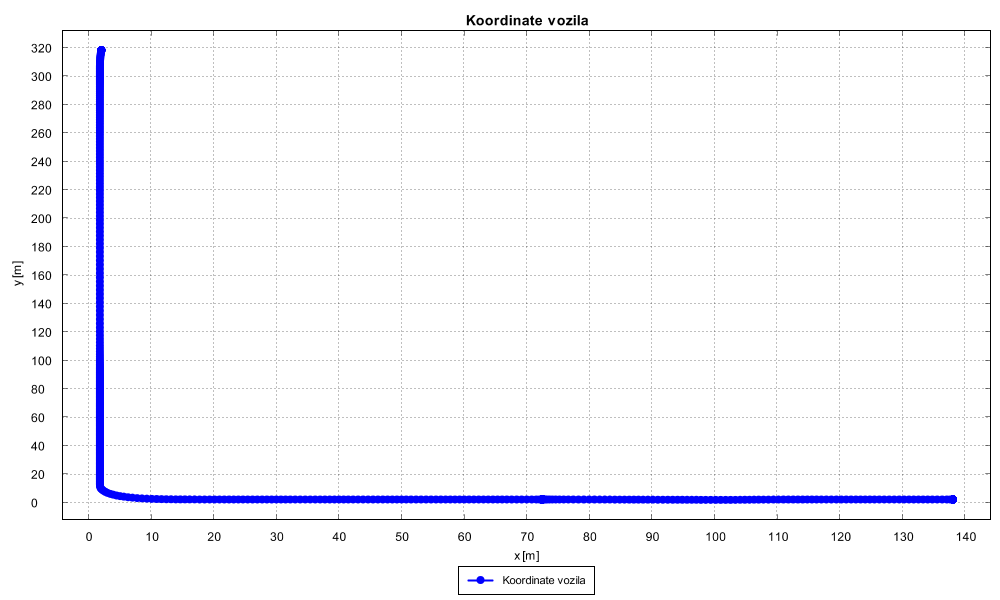
\includegraphics[scale=0.35]{images/koordinate2.png}
  \caption{Graf lokacije vozila}
  \label{fig:gt2_lokacija}
\end{figure}
\begin{figure}[H]
  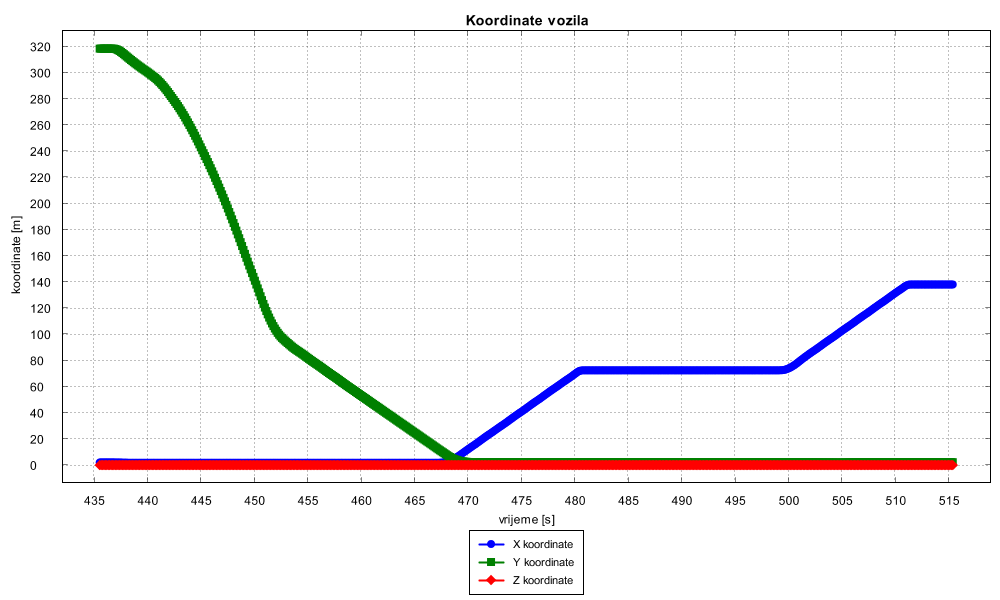
\includegraphics[scale=0.35]{images/koordinate_vrijeme2.png}
  \caption{Graf x, y i z koordinata vozila u vremenu}
  \label{fig:gt2_lokacija_koord}
\end{figure}
\begin{figure}[H]
  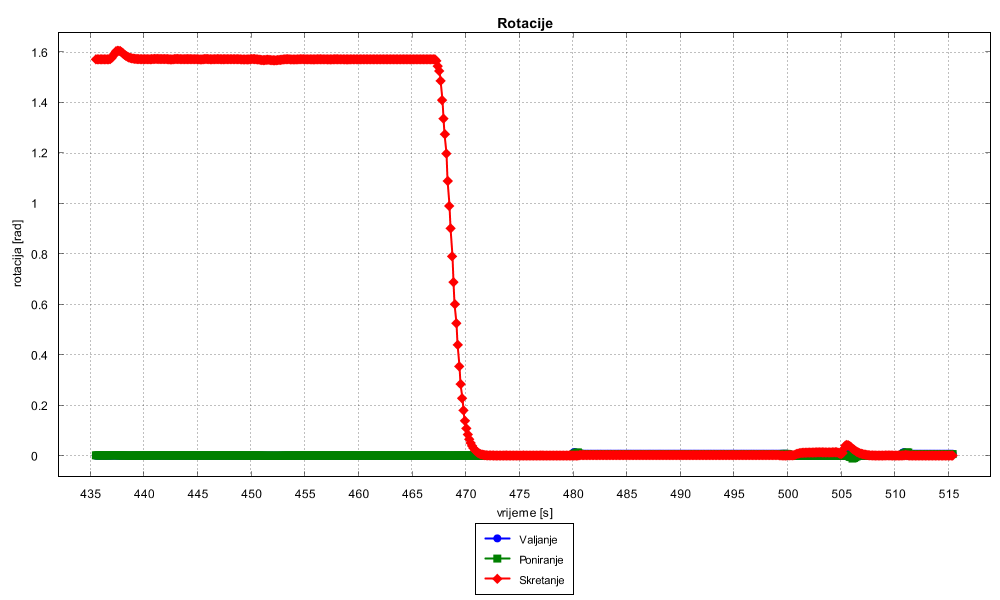
\includegraphics[scale=0.35]{images/rotacija_vrijeme2.png}
  \caption{Valjanje, skretanje i poniranje vozila u vremenu}
  \label{fig:gt2_rot_vr}
\end{figure}
\begin{figure}[H]
  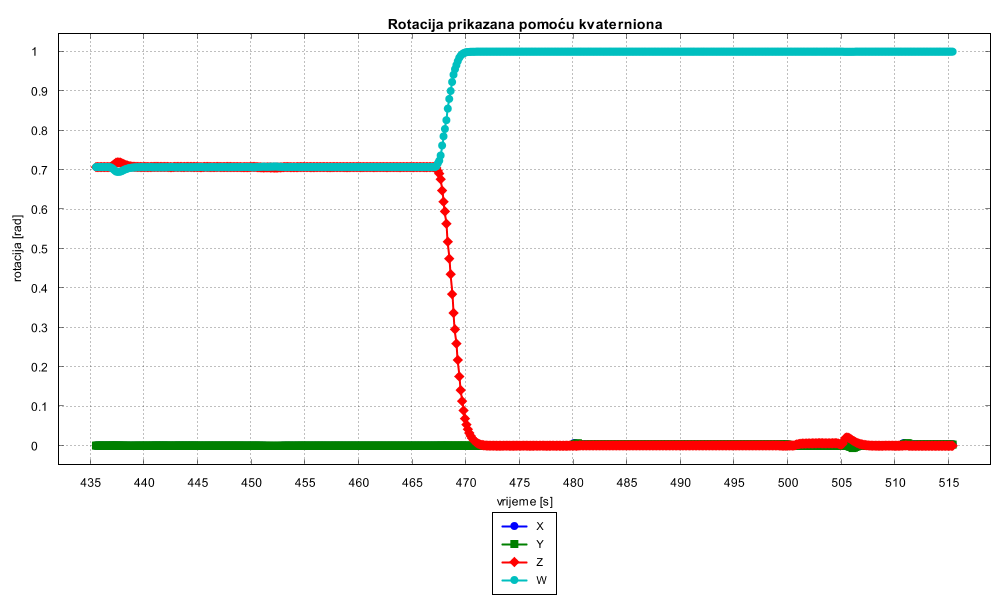
\includegraphics[scale=0.35]{images/rotacija_kvaterni2.png}
  \caption{Rotacija vozila u obliku kvaterniona}
  \label{fig:gt2_rot_kv}
\end{figure}
Prvi niz skupova točaka se skupljao u dužem periodu ali ima samo 300 skupova zato što se koristi svako 15 očitanje. Drugi niz skupova točaka ima 600 očitanja zato što se uzima svako očitanje. Također je drugi skup detaljniji od prvoga što pridonosi točnosti algoritama. Duljinu puta možemo izračunati tako da pronađemo udaljenosti između dvije sljedne točke te ih zbrojimo. Tako dobivena udaljenost za referentni primjer A iznosi 662.3 metra, a za referentni primjer B iznosi 448.2 metra.

\begin{listing}[H]
  \begin{minted}[frame=lines, linenos]{text}
void save_matrix(ICP icp, string first, string second) {
 Matrix4d transformation = icp.getFinalTransformation();
 double fitness = icp.getFitnessScore();
 string filename = first + "-" + second + ".txt";
 Matrix3d mat = mat4x4_to_3x3(transformation);
 Vector3d rpy = mat.eulerAngles(0, 1, 2);
 save_to_file(
   filename,
   mat_to_string(transformation),
   fitness,
   rpy
  );
}
  \end{minted}
  \caption{Generalizirani ICP - spremanje rezultata}
  \label{coderef:gen_icp_save_matrix}
\end{listing}

Spremanje rezultata se vrši metodom \mintinline{text}{save_matrix} u primjeru \ref{coderef:gen_icp_save_matrix}. Matricu transformacije možemo dobiti pozivom \mintinline{text}{icp.getFinalTransformation()} te je  oblika \mintinline{text}{Matrix4d} tj. ima 4 redaka i 4 stupaca dok su elemnti tipa \mintinline{text}{double}. Ta matrica se tada transformira u matricu veličine 3x3 tj. izdvaja se rotacijska matrica zato što takav tip matrice ima ugrađenu metodu \mintinline{text}{eulerAngles()}. Ta metoda kao argumente prima redosljed rotacija objekta tj. redosljed osi rotacija. U ovome slučaju se prvo predaje 0 što znači da se objekt prvo rotirao oko x osi, tada se predaje 1 što znači da se tada rotirao oko y osi i naposljetku se predaje 2 što znači da je zadnja rotacija bila oko z osi. Metoda vraća vektor od tri elementa koji predstavljaju valjanje, poniranje i skretanje. Konačno se sve te informacije spremaju u datoteku s imenom sastavljenim od dva indetifikatora očitanja tako da se zna koji skupovi točaka su upoređivani. Struktura te datoteke je prikazana na primjeru  \ref{files:icp_file_result}. Prva linija sadrži fitnes vrijednost. Od druge do pete linije se nalazi transformacijska matrica dok se na zadnjoj liniji nalaze Eulerovi kutevi u radijanima.
\begin{listing}[H]
  \begin{minted}[frame=lines]{text}
0.0263544
    0.999735   -0.0230172  -0.00046344  -0.00394583
   0.0230173     0.999735  0.000237121  0.000806379
 0.000457859 -0.000247725            1    0.0091155
           0            0            0            1
3.14136 -3.14113 -3.11857
  \end{minted}
  \caption{ICP - datoteka s rezultatom}
  \label{files:icp_file_result}
\end{listing}

\begin{equation}
  \begin{aligned}
AM_{x} &= \frac{1}{n}\sum_{i=0}^{n-1} |X_{i} - \hat{X}_{i}|\\
AM_{y} &= \frac{1}{n}\sum_{i=0}^{n-1} |Y_{i} - \hat{Y}_{i}|\\
AM_{z} &= \frac{1}{n}\sum_{i=0}^{n-1} |Z_{i} - \hat{Z}_{i}|
  \end{aligned}
  \label{eq:coord_am}
\end{equation}
\begin{equation}
  \begin{aligned}
MSE_{x} &= \frac{1}{n}\sum_{i=0}^{n-1} |X_{i} - \hat{X}_{i}|^2\\
MSE_{y} &= \frac{1}{n}\sum_{i=0}^{n-1} |Y_{i} - \hat{Y}_{i}|^2\\
MSE_{z} &= \frac{1}{n}\sum_{i=0}^{n-1} |Z_{i} - \hat{Z}_{i}|^2
  \end{aligned}
  \label{eq:coord_mse}
\end{equation}

\begin{equation}
  \begin{aligned}
ROT_{r} &= \frac{1}{n}\sum_{i=0}^{n-1} |R_{i} - \hat{R}_{i}|\\
ROT_{p} &= \frac{1}{n}\sum_{i=0}^{n-1} |P_{i} - \hat{P}_{i}|\\
ROT_{y} &= \frac{1}{n}\sum_{i=0}^{n-1} |Y_{i} - \hat{Y}_{i}|
  \end{aligned}
  \label{eq:rot_am}
\end{equation}
\begin{equation}
  \begin{aligned}
ROT_{r} &= \frac{1}{n}\sum_{i=0}^{n-1} |R_{i} - \hat{R}_{i}|^2\\
ROT_{p} &= \frac{1}{n}\sum_{i=0}^{n-1} |P_{i} - \hat{P}_{i}|^2\\
ROT_{y} &= \frac{1}{n}\sum_{i=0}^{n-1} |Y_{i} - \hat{Y}_{i}|^2
  \end{aligned}
  \label{eq:rot_mse}
\end{equation}


Konkretnije numeričke estimacije i pogreške se računaju pomoću sljedećih formula. Sretnja aritmetička vrijednosti razlika koordinata i rotacija se računa s formulama \ref{eq:coord_am} i \ref{eq:rot_am}. Element $n$ je ukupan broj točaka, $X_{i}$ je stvarna vrijednost koordinate x, dok je $\hat{X}_{i}$ estimirani iznos x koordinate. Po istome principu vrijedi za x i y koordinate. Element $R_{i}$ je stvarna vrijednost kuta valjanja, dok je $\hat{R}_{}$ estimirana vrijednost kuta valjanja. Po istome principu vrijedi za skretanje i poniranje. Srednje kvadratične pogreška koordinata i rotacije se računaju s formulama \ref{eq:coord_mse} i \ref{eq:rot_mse}. AM znači aritmetička sredina razlika, dok MSE znači srednja kvadratična pogreška. Prilikom računanja srednjih pogrešaka kuteva, a tako i razlike kuteva, uzeta je periodičnost kuteva u obzir.
\pagebreak